\subsubsection{Introduction}
Many relevant biological processes, such as transmembrane permeation or transitions between active and inactive protein conformations, occur on a $\mu$s-s timescale\cite{Zwier2010,Choy2017,Wells2007}. However, even with GPU acceleration, the timescales accessible via molecular dynamics (MD) simulations are only a few hundred ns/day\cite{HecBioSim_benchmark}. One of the methods to get around this limitation is steered molecular dynamics (sMD). sMD involves applying a harmonic restraint to bias the system towards a conformation defined through one or more collective variables (CVs):

\begin{equation}
V(\vec{s},t) = \frac{1}{2} \kappa(t) ( \vec{s} - \vec{s}_0(t) )^2
\label{eq:sMD}
\end{equation}

where $\kappa$ is the force constant, $\vec{s}_0$ is the expected CV value at a specific timestep, and $\vec{s}$ is the actual CV value at that timestep\cite{Isralewitz2001,Tribello2014}.

This section of the tutorial involves using BioSimSpace to set up and run sMD simulations. BSS prepares input files for PLUMED, which is the software that works together with MD engines such as AMBER and GROMACS to add the restraint in eq \ref{eq:sMD}.

The protein that will be used as an example in this tutorial is protein tyrosine phosphatase 1B (PTP1B). It is a negative regulator of insulin signalling\cite{sMD_ptp1b-diabetes} and is an attractive target for type II diabetes\cite{sMD_Wiesman}. The function of PTP1B depends on the conformation of its WPD loop, which can be closed (active) or open (inactive) (Figure \ref{fig:ptp1b}). The WPD loop of PTP1B opens and closes on a $\mu$s timescale\cite{Choy2017}, and therefore this transition is not observed on conventional computational timescales.

\begin{figure}[htp]
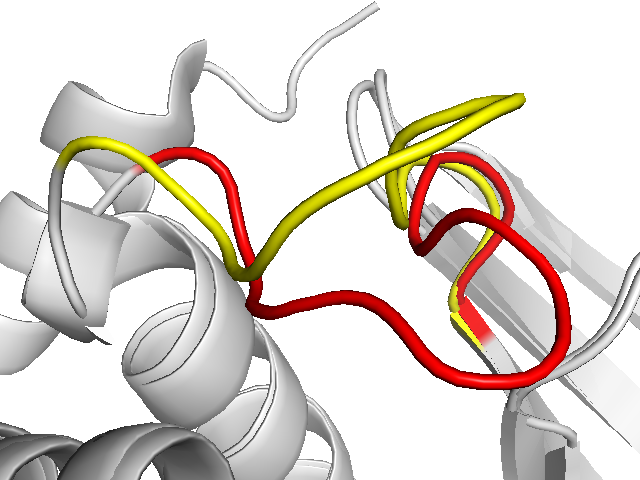
\includegraphics[width=\linewidth]{LIVECOMS/03_steered_md/open-close.png}
\caption{The WPD loop of PTP1B, in two conformations: open (yellow, PDB ID: 2HNP) and closed (red, PDB ID: 1SUG).}
\label{fig:ptp1b}
\end{figure}

\subsubsection{Running sMD using BioSimSpace}

The first notebook of this tutorial \href{https://github.com/OpenBioSim/BioSimSpaceTutorials/blob/main/03_steered_md/01_setup_sMD.ipynb}{01-setup-sMD} describes how to setup a steered MD simulation with BioSimSpace. 
The notebook illustrates the use of \href{https://biosimspace.openbiosim.org/api/generated/BioSimSpace.Metadynamics.CollectiveVariable.RMSD.html#BioSimSpace.Metadynamics.CollectiveVariable.RMSD}{BSS.Metadynamics.CollectiveVariable.RMSD} to define a collective variable that enforces a conformational change of the 'WPD' loop in the enzyme PTP1B. 
Next \href{https://biosimspace.openbiosim.org/api/generated/BioSimSpace.Protocol.Steering.html#BioSimSpace.Protocol.Steering}{BSS.Protocol.Steering} is used to specific a steering schedule alongside the RMSD CV. The notebook illustrates how input files for the gmx, sander or pmemd MD engines can be subsequently prepared. The notebook also shows how more complex steering schedule that combine multiple CVs can be specified. 

For production simulations we recommend long sMD simulations to minimise the strength of the bias that needs to be applied to enforce the desired conformational change by the end of the steered MD simulation. Optimising the steered MD schedule parameters requires trial and error. 
For convenience we provide simple python scripts with a command line interface to execute steered MD runs and scan schedule parameters for two specified sMD protocol (\href{https://github.com/OpenBioSim/BioSimSpaceTutorials/blob/main/03_steered_md/scripts/sMD_simple.py}{a single CV} and a \href{https://github.com/OpenBioSim/BioSimSpaceTutorials/blob/main/03_steered_md/scripts/sMD_multiCV.py}{multiple CV} example). We also provide sample \href{https://github.com/OpenBioSim/BioSimSpaceTutorials/blob/main/03_steered_md/scripts/sMD_slurm.sh}{slurm} and \href{https://github.com/OpenBioSim/BioSimSpaceTutorials/blob/main/03_steered_md/scripts/sMD_LSF.sh}{LSF} submission scripts to deploy the BSS steered MD scripts in different HPC environments. 

\subsubsection{sMD trajectory analysis}

The second notebook of this tutorial \href{https://github.com/OpenBioSim/BioSimSpaceTutorials/blob/main/03_steered_md/02_trajectory_analysis.ipynb}{02-trajectory-analysis} describes how to analyse data generated by a steered MD run. As the sMD simulation is run, the CV values are saved to a \textbf{COLVAR} file. It can be plotted to assess whether the sMD simulation has been successful. An example is shown in Figure \ref{fig:rmsd}.

\begin{figure}[htp]
    \centering
    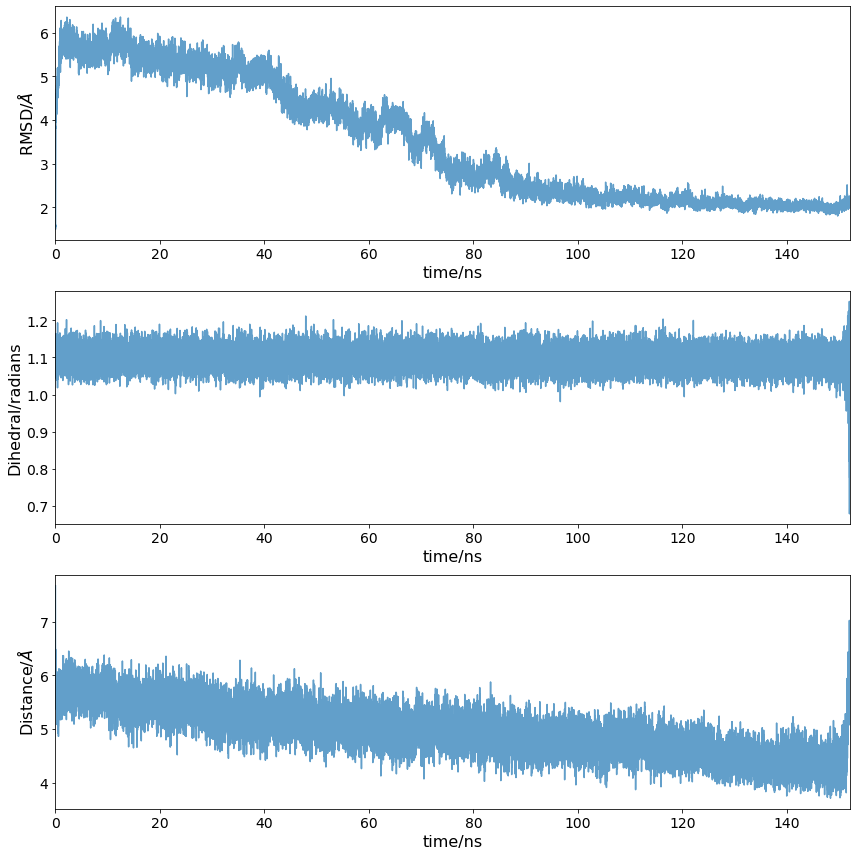
\includegraphics[width=\linewidth]{LIVECOMS/03_steered_md/COLVAR_all.png}
    \caption{RMSD change throughout an sMD simulation. As the simulation progresses, the WPD loop RMSD gets closer and closer to the closed loop crystal structure (i.e. the loop is being closed).}
    \label{fig:rmsd}
\end{figure}

The notebook also illustrates a "failed" steered MD trajectory, where the steering duration and force were insufficient to reach the target CV value.

\subsubsection{Markov State Models}
While the information provided here focuses on running sMD simulations with BSS, there are multiple potential applications, such as studying permeability of membranes\cite{Wells2007} or ligand residence time\cite{Potterton2019}. Another use is additional exploration of conformational space for predicting allosteric modulation using Markov State Models (MSMs). MSMs give the probability of protein conformations, and therefore can be used to model how a ligand affects the conformation ensemble of a target (e.g. whether it decreases the active state probability and therefore is an allosteric inhibitor). There is a lot to consider when building MSMs, and the method is not covered in this tutorial. Here the python library \href{http://emma-project.org/latest/}{PyEMMA} was used, which has extensive examples and documentation\cite{Wehmeyer_2019}. The integration of sMD in this allosteric modulation prediction workflow is illustrated in Figure \ref{fig:ensemble-protocol}. \href{https://github.com/OpenBioSim/BioSimSpaceTutorials/blob/main/03_steered_md/02_trajectory_analysis.ipynb}{02-trajectory-analysis} shows how the sMD trajectory can be sampled to extract a range of protein conformations. Hardie \emph{et al} report a detailed study of allosteric modulators of PTP1B using this sMD/MSM methodology\cite{Hardie2023}.

\begin{figure}[htp]
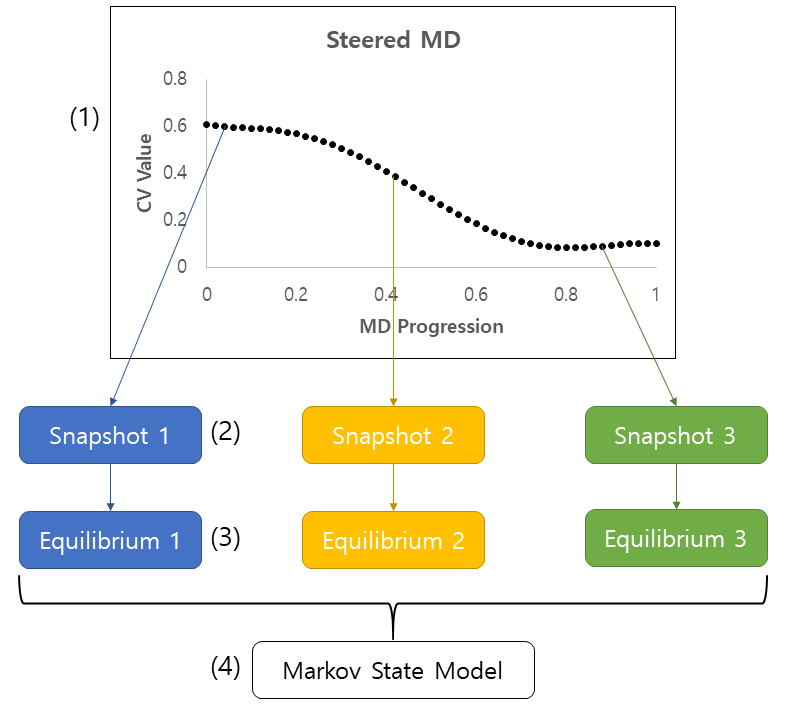
\includegraphics[width=\linewidth]{LIVECOMS/03_steered_md/ensemble-md-protocol.png}
\caption{The steps of using enhanced sampling methods to gather data for statistical analysis of protein conformation ensemble. (1) Run steered MD along some collective variable (CV); (2) Extract snapshots that evenly sample available conformational space; (3) Run equilibrium MD simulations using extracted coordinates as seeds; (4) construct an MSM using trajectory data from step 3.}
\label{fig:ensemble-protocol}
\end{figure}